\documentclass[conference]{IEEEtran}
\IEEEoverridecommandlockouts
% The preceding line is only needed to identify funding in the first footnote. If that is unneeded, please comment it out.
\usepackage{cite}
\usepackage{amsmath,amssymb,amsfonts}
\usepackage{algorithmic}
\usepackage{graphicx}
\usepackage{textcomp}
\usepackage{graphicx}
\graphicspath{ {./images/} }
\usepackage{xcolor}
\usepackage[utf8]{inputenc}
\usepackage{hyperref}
\def\BibTeX{{\rm B\kern-.05em{\sc i\kern-.025em b}\kern-.08em
    T\kern-.1667em\lower.7ex\hbox{E}\kern-.125emX}}
\begin{document}

\title{
Knight's tour Problem \\
}

\author{\IEEEauthorblockN{Kalpana Khutela}
\IEEEauthorblockA{IIB2019019}
\and
\IEEEauthorblockN{Devang Bharti}
\IEEEauthorblockA{IIB2019020}
\and
\IEEEauthorblockN{Hitka Rajesh Kumar }
\IEEEauthorblockA{IIB2019021}
}

\maketitle

\noindent \begin{abstract}

In this report we used modified backtracking approach to solve the knight's tour problem \\\\
Keyword : backtracking, time complexity, space complexity.

\end{abstract}


\section{\textbf{Introduction}}
\noindent In this problem, we have to propose a algorithm to solve knight's tour problem \\\\

\noindent we have given a brief idea of our algorithm \textbf{part II}.\\


\section{\textbf {Algorithm Approach}}

\begin{enumerate}

\item A BLOCK OF THE CHESS ‘B’ CAN BE TAKEN INTO FURTHER MOVE OF THE KNIGHT FROM BLOCK ‘A’ IF:\\

‘B’ IS UNVISITED.
‘B’ CAN BE REACHED BY A SINGLE MOVE OF THE KNIGHT.
\\

\item ASSUME ‘A’ TO BE THE RANDOM INITIAL  POSITION FROM WHERE THE KNIGHT STARTS IT TRAVEL.\\

\item SINCE ‘A’ IS VISTED IT IS NEEDED TO  MARK IT WITH “1”.
\\
\item TO MOVE TO ANY POSITION ‘B’ FROM ‘A’\\
\item LET A SET ‘S’ HAVE ALL THE POSSIBLE POSITIONS WHICH CAN BE REACHED FROM ‘A’.
\item FROM THIS SET ‘S’ CHOOSE THE PATH WHICH IS HAVING MINIMUM ONWARD MOVES.\\
\item AFTER BEING CHOSEN MARK IT ‘2’ \\
\item THIS IS THE MAIN LOGIC BEHIND THIS PROBLEM AND THIS GOES ON FURTHER .\\

\textbf{For Example - }

Let input be\\
for the position (0,0)\\

There are 8 points (1,2) (2,1) (2,-1) (1, -2) (-1,-2) (-2,-1) (-2,1) and (-1,2).\\
In 8 points (2,-1) (1, -2) (-1,-2) (-2,-1) (-2,1) (-1,2) points are invalid\\
So we have to go either (1,2) or (2,1).\\
We will choose any of them and then from that point will see the next 8 points and consider only the valid moves.\\
If at any position no possible move will not possible then back to the previous move and from that go to the other path and stop if the step cont will be 64.\\
\end{enumerate}


\section{\textbf{Pseudo Code I}} 
\noindent Function isValid \\
Pass :int x, int y\\
\bef\begin{algorithmic}
	\IF{$((x>=0 and y>=0) and (x<N and y<N))$}\\
    	return true\\
	\ENDIF\\
retun False\\
\end{algorithmic}


\section{\textbf{Pseudo Code II}} 
\noindent Function isEmpty \\
Pass :int  result[], int x, int y\\
\begin{algorithmic}
  	return (isValid(x, y)) && (result[y*N+x] < 0);
\end{algorithmic}


\section{\textbf{Pseudo Code III}} 
\noindent Function int degree \\
Pass :nit result[], int x, int y\\
\begin{algorithmic}
\STATE $int count =0$\\ 
	\for{$int i=0$ to $N$}\\
	\IF {$IsEmpty(result,x+nextx[i],y+nexty[i])$}
	\STATE$cunt=count+1$\\
	return count
		
\end{algorithmic}


\section{\textbf{Pseudo Code IV}} 
\noindent Function FindNMove \\
Pass : int result[], int x, int y\\
\begin{algorithmic}
    \STATE $int min_deg_index =-1,c,min_deg=(N+1),nx,ny$
	\STATE $int start\gets rand()\bmod N$\\
	 \For{$count \gets 0$ to $N$}
	    \STATE {$ int i=(start+count)\bmod N$}
	    \STATE $nx=*x+next_x[i]$
	    \STATE $ny=*y+next_y[i]$
	    \IF{$isEmpty(result ,nx, ny) and                     c=degree(result,nx,ny)< mindeg$}
            \STATE $minimum index =i$
            \STATE $min degree =c$
        \ENDIF
    \ENDFOR\\
    \IF{$mindegindex==-1$} 
    return FALSE\\
    \STATE $nx =*x+nextx[mindegindex]$\\
    \STATE $ny =*x+nexty[mindegindex]$\\
    \STATE $result[ny*N+nx]=result[(*y)*N+(*x)]+1$\\
    \STATE $*x=nx$\\
    \STATE $*y=ny$\\
    return TRUE
\end{algorithmic}


\section{\textbf{Pseudo Code V}} 
\noindent Function Print result \\
Pass : int result[]\\
\begin{algorithmic}
 \For{$i=0$ to$N$}\\
   \For{$j=0$ to$N$}\\
     $Print result[j*N+1]$\\
    \ENDFOR
  \ENDFOR   
\end{algorithmic}


\section{\textbf{Pseudo Code VI}} 
\noindent Function bool checkNeighbour \\
Pass :int x, int y, int xx, int yy\\
\begin{algorithmic}
  \for{$(int i=0$) to $N$}
		\IF{$(((x+nextx[i]) == xx)&&((y + nexty[i]) == yy))$}
			return true\\
	return false\\
\end{algorithmic}
\section{\textbf{Pseudo Code VII}} 
\noindent Function bool knightTour \\
\begin{algorithmic}

	\STATE$int result[N*N]$
	\for{$int i=0;$ to $N*N$} 
		\STATE $result[i] = -1$
	    \STATE $int sx,sy$
	 \STATE $cin>> sx >> sy$
	 \STATE$int x = sx, y = sy$
	\STATE$result[y*N+x] = 1$ 

	\for{$int i=0$ to $N*N-1$}
		\IF{$(findNmove(result,&x,&y) == 0)$}\\
			return false\\
        \IF{(!checkNeighbour(x,y,sx,sy))}
		return false\\
    \STATE $printResult(result)$\\
	return true\\
\end{algorithmic}


\section{\textbf {Time Complexity}}
\noindent the time needed for this algorithm grows roughly linearaly with the number of squares of the chessboard that is pow(n,2).
\begin{figure}[htp]
    \centering
    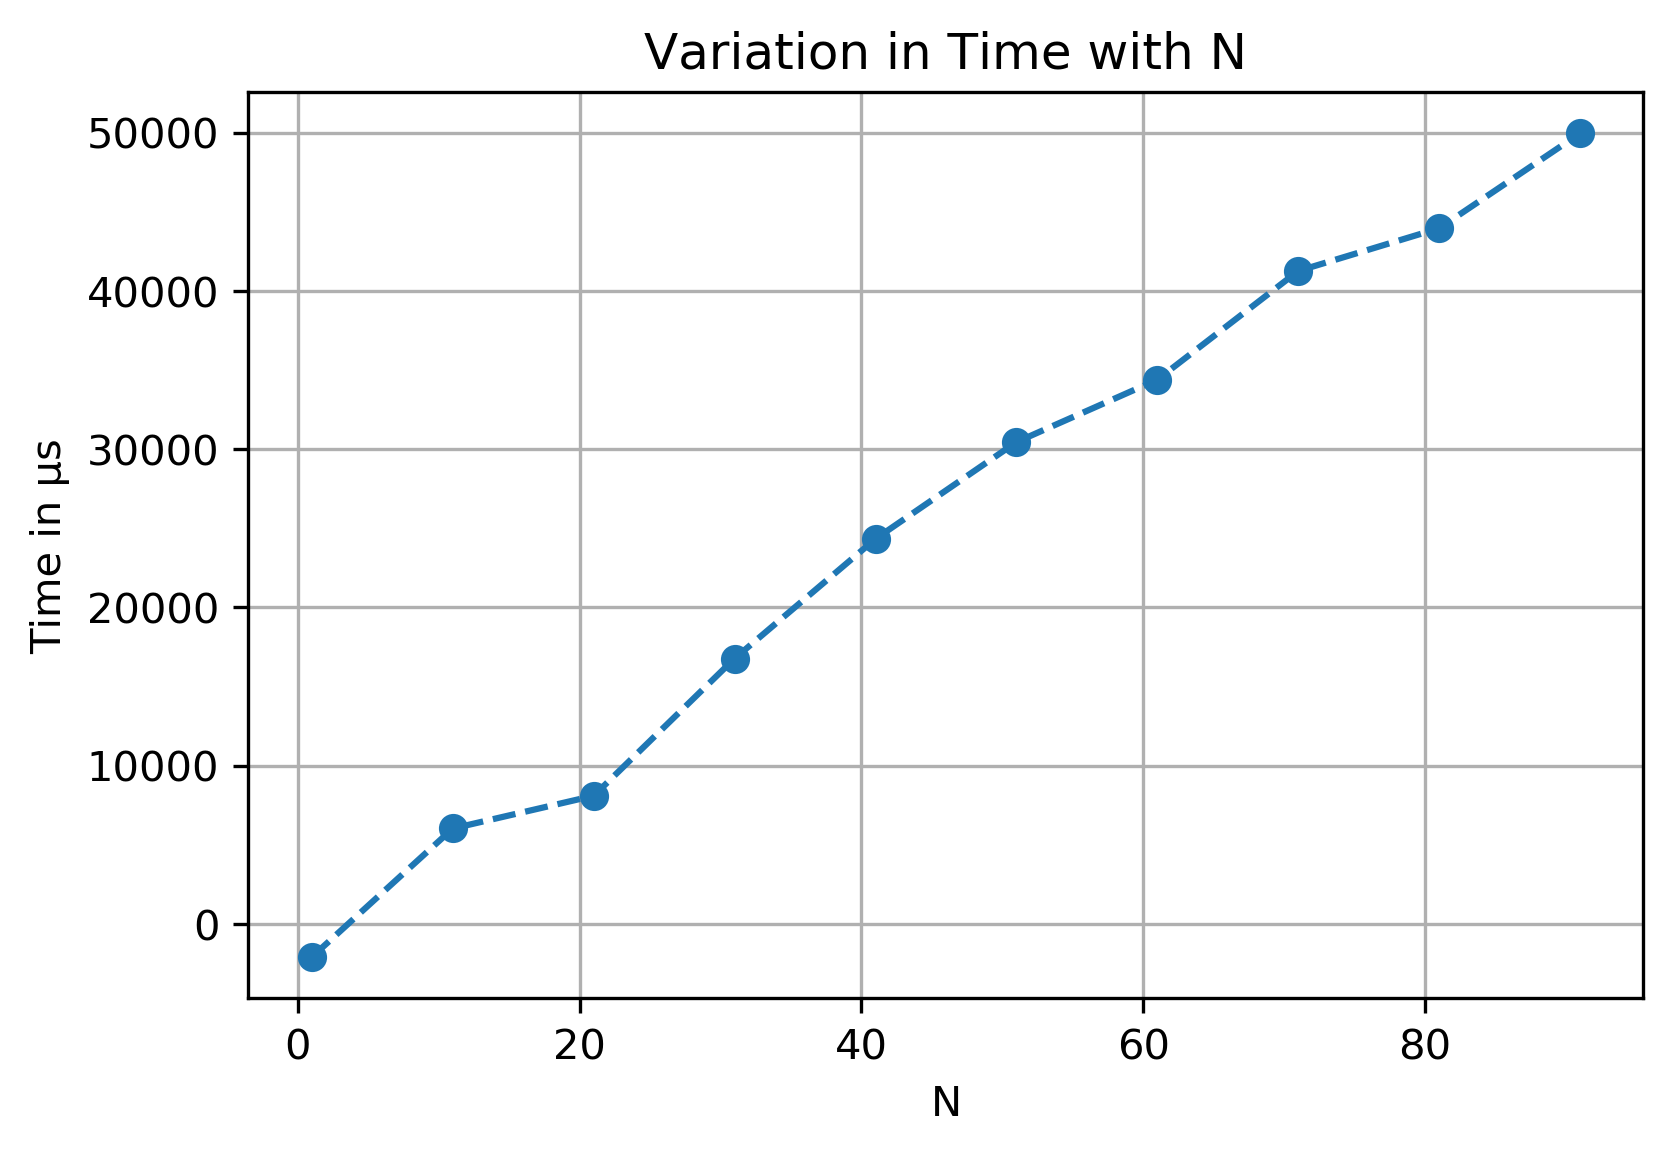
\includegraphics[width=8cm]{time_com}
    \caption{Time complexity curve}
    \label{fig:time_com.png}
\end{figure}

\section{\textbf {Auxiliary Space Complexity}}
\noindent No extra space is used in this algorithm, so auxiliary space is of order pow(n,2).Only the input array is of size n*n.
Space Complexity = Input Space+Auxiliary Space, which is equal to pow(n,2).


\begin{figure}[htp]
    \centering
    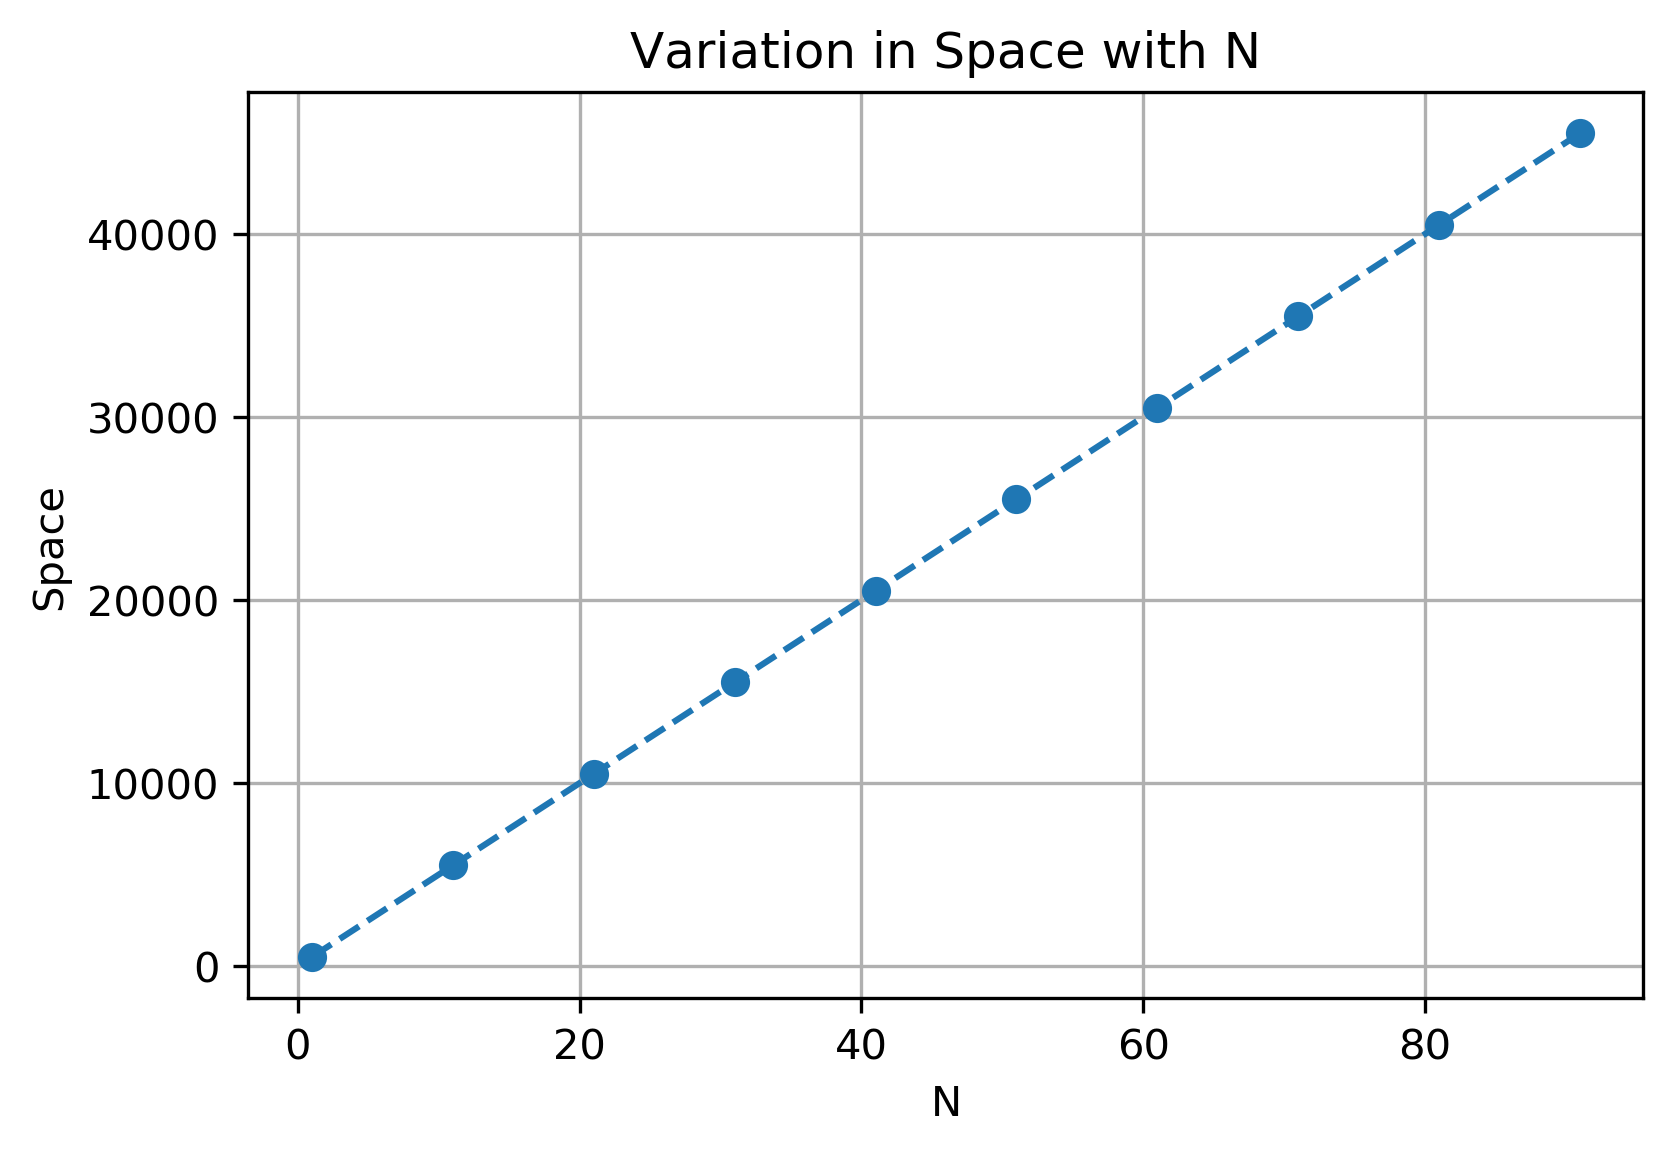
\includegraphics[width=8cm]{Aux_space}
    \caption{Auxiliary space complexity curve}
    \label{fig:Aux_space.jpeg}
\end{figure}

\section{\textbf {Conclusion}} \noindent The above proposed algorithm efficiently gives whether it can cover the board or not. The algorithm proposed is very efficient both space and time wise \\
\section{\textbf {References}} 
\begin{enumerate}

\item  \href{https://stackoverflow.com/questions/19214109/how-to-optimize-knights-tour-algorithm}{optimization of knight and tour algorithm}\\
    
\item  \href{https://www.geeksforgeeks.org/warnsdorffs-algorithm-knights-tour-problem/}{
Knight's tour algorithm}
\\

\end{enumerate}

\end{document}